\documentclass[11pt,a4paper]{article}

\usepackage{epsfig}
\usepackage{multicol}

\usepackage[utf8]{inputenc}
\usepackage[brazil]{babel}
\usepackage{fancyheadings}
\usepackage{amsmath}
\usepackage{calrsfs}
\usepackage{enumerate}
\DeclareGraphicsExtensions{.png,.pdf}
\usepackage{amsmath, amsfonts, amssymb}
\usepackage{esint}
\usepackage{graphicx}
\usepackage{multicol}
\usepackage{tasks}
\usepackage[utf8]{inputenc}
\usepackage{mathrsfs} % Transformada de Laplace
\usepackage{indentfirst}

% As margens
\setlength{\textheight}{24.0cm}
\setlength{\textwidth}{17.5cm}
\setlength{\oddsidemargin}{2.0cm} % Margens reais desejadas
\setlength{\evensidemargin}{2.0cm} % 2+17.5+1.5=21cm (largura A4)
\setlength{\topmargin}{1.5cm} % 1.5+1.6+1.0+24.0+1.6=29.7cm
\setlength{\headheight}{1.6cm} % (altura A4)
\setlength{\headsep}{1.0cm}
\setlength{\columnsep}{1.5cm} % Coluna = 8cm ((17.5-1.5)/2)
\addtolength{\oddsidemargin}{-1in}
\addtolength{\evensidemargin}{-1in}
\addtolength{\topmargin}{-1in}
\setlength{\footskip}{0.0cm}


% Novos comandos
\newcommand{\limite}{\displaystyle\lim}
\newcommand{\integral}{\displaystyle\int}
\newcommand{\somatorio}{\displaystyle\sum}
\newcommand{\mat}[1]{\mbox{\boldmath{$#1$}}} 

\pagestyle{fancy}


\usepackage{lipsum}

\lhead{

\includegraphics[width=1cm]{brasao.png}
}

\rhead{ 
\sc\textbf{U}niversidade \textbf{F}ederal do \textbf{C}eará\\
Campus Quixadá\\ Monitoria de Cálculo II e III}

\cfoot{}

\begin{document}

	\begin{center}
		\Large Lista 3 - Cálculo III
	\end{center}
	

	\begin{enumerate}
		\item Calcule o volume do conjunto dado.
			\begin{enumerate}
				\item $\{(x,y,z) \in \mathbb{R}^3 \,|\, 0 \leq x \leq 1\ \textrm{,}\ 0 \leq y \leq 1\ \textrm{,}\ 0 \leq z \leq x + 2y\}$.	
				\item $\{(x,y,z) \in \mathbb{R}^3 \,|\, 0 \leq x \leq 2\ \textrm{,}\ 1 \leq y \leq 2\ \textrm{,}\ 0 \leq z \leq \sqrt{xy}\}$.
				\item $\{(x,y,z) \in \mathbb{R}^3 \,|\, 0 \leq x \leq 1\ \textrm{,}\ 0 \leq y \leq 1\ \textrm{,}\ 0 \leq z \leq xye^{x^2 - y^2}\}$.
				\item $\{(x,y,z) \in \mathbb{R}^3 \,|\, 0 \leq x \leq 1\ \textrm{,}\ 0 \leq y \leq 1\ \textrm{,}\ x^2 + y^2 \leq z \leq 2\}$.
				\item $\{(x,y,z) \in \mathbb{R}^3 \,|\, 1 \leq x \leq 2\ \textrm{,}\ 0 \leq y \leq 1\ \textrm{,}\ x + y \leq z \leq x + y + 2\}$.
				\item $\{(x,y,z) \in \mathbb{R}^3 \,|\, 0 \leq x \leq 1\ \textrm{,}\ 0 \leq y \leq 1\ \textrm{,}\ 1 \leq z \leq e^{x + y}\}$.
			\end{enumerate}
			
		\item Calcule $\displaystyle\iint_B y \,dx\,dy$ onde B é o conjunto dado.
		
		\begin{enumerate}
			\item $B$ é o triângulo de vértices $(0,0),(1,0) \textrm{ e } (1,1)$.
			\item $\{(x,y) \in \mathbb{R}^2 \,|\, -1 \leq x \leq 1\ \textrm{,}\ 0 \leq y \leq x + 2\}$.
			\item $B$ é o conjunto de todos $(x,y)$ tais que $x^2 + 4y^2 \leq 1$.
			\item $B$ é o triângulo de vértices $(0,0),(1,0) \textrm{ e } (2,1)$.
			\item $B$ é a região compreendida entre os gráficos de $y = x$ e $y = x^2$, com $0 \leq x \leq 2 $.
			\item $B$ é o paralelogramo de vértices $(-1,0),(0,0),(1,1) \textrm{ e } (0,1)$.
			\item $B$ é o semicírculo $x^2 + y^2 \leq 4$, $y \geq 0$.
			\item $\{(x,y) \in \mathbb{R}^2 \,|\, x \geq 0\ \textrm{,}\ x^5 - x \leq y \leq 0\}$.
		\end{enumerate}
		
		\item Calcule $\displaystyle\iint_B f(x,y) \,dx\,dy$ sendo dados:
		\begin{enumerate}
			\item $f(x,y) = x \cos y$ e $B = \{(x,y) \in \mathbb{R}^2 \,|\, x \geq 0\ \textrm{,}\ x^2 \leq y \leq \pi \}$.
			\item $f(x,y) = xy$ e $B = \{(x,y) \in \mathbb{R}^2 \,|\, x^2 + y^2 \leq 2\ \textrm{,}\ y \leq x  \textrm{ e } x \geq 0 \}$.
			\item $f(x,y) = x$ e $B$ é o triângulo de vértices $(0,0),(1,1) \textrm{ e } (2,0)$.
			\item $f(x,y) = xy \cos x^2$ e $B = \{(x,y) \in \mathbb{R}^2 \,|\, 0 \leq x \leq 1\ \textrm{,}\ x^2 \leq y \leq 1\}$.
			\item $f(x,y) = x + y$ e $B$ a região compreendida entre os gráficos das funções $y = x$ e $y = e^x$, com $0 \leq x \leq 1$.
			\item $f(x,y) = x^5 \cos y^3$ e $B = \{(x,y) \in \mathbb{R}^2 \,|\, y \geq x^2\ \textrm{,}\ x^2 + y^2 \leq 2 \}$. 
			\item $f(x,y) = x$ e $B$ a região compreendida entre os gráficos de $y = cox$ e $y = 1 - \cos x$, com $0 \leq x \leq \dfrac{\pi}{2}$.
			\item $f(x,y) = \sqrt{1 + y^3}$ e $B = \{(x,y) \in \mathbb{R}^2 \,|\, \sqrt{x} \leq y \leq 1 \}$.
			\item $\displaystyle\dfrac{y}{x^2 + y^2}$ e $B$ o conjunto de todos $(x,y)$ tais que $1 \leq x \leq 4$ e $0 \leq x \leq \sqrt{x}$.
			
		\end{enumerate}
		\item Inverta a ordem de integração.
		
		\begin{enumerate}
			\item $\integral_0^{1} \left[ \integral_0^{x} f(x,y) \, dy \right] dx$.
			\item $\integral_0^{1} \left[ \integral_{x^2}^{x} f(x,y) \, dy \right] dx$.
			\item $\integral_0^{1} \left[ \integral_{-\sqrt{y}}^{\sqrt{y}} f(x,y) \, dx \right] dy$.
			\item $\integral_1^{e} \left[ \integral_{\ln x}^{x} f(x,y) \, dy \right] dx$.
			\item $\integral_0^{1} \left[ \integral_y^{y+3} f(x,y) \, dx \right] dy$.
			\item $\integral_{-1}^{1} \left[ \integral_{-\sqrt{1-x^2}}^{\sqrt{1-x^2}} f(x,y) \, dy \right] dx$.
			\item $\integral_{-1}^{1} \left[ \integral_{x^2}^{\sqrt{2-x^2}} f(x,y) \, dy \right] dx$.
			\item $\integral_0^{1} \left[ \integral_{y-1}^{2-2y} f(x,y) \, dx \right] dy$.
			\item $\integral_0^{1} \left[ \integral_{x^2}^{1} f(x,y) \, dy \right] dx$.
			\item $\integral_0^{1} \left[ \integral_{e^{y-1}}^{e^y} f(x,y) \, dx \right] dy$.
			\item $\integral_0^{1} \left[ \integral_{2x}^{x+1} f(x,y) \, dy \right] dx$.
			\item $\integral_0^{1} \left[ \integral_{\sqrt{x-x^2}}^{\sqrt{2x}} f(x,y) \, dy \right] dx$.
			\item $\integral_0^{\pi} \left[ \integral_0^{\sin x} f(x,y) \, dy \right] dx$.
			\item $\integral_0^{\pi/4} \left[ \integral_{\sin x}^{\cos x} f(x,y) \, dy \right] dx$.
			\item $\integral_{-1}^{2} \left[ \integral_{\sqrt{(7+5y^2)/3}}^{(y+7)/3} f(x,y) \, dx \right] dy$.
			
		\end{enumerate}
		
		\item Calcule o volume do conjunto dado. (Desenhe o conjunto para facilitar mais a visualização.)
		
		\begin{enumerate}
			\item $x^2 + y^2 \leq 1$ e $x+y+2 \leq z \leq 4$.
			\item $x \geq 0$, $y \geq 0$, $x+y \leq 1$ e $0 \leq z \leq x^2 + y^2$.
			\item $0 \leq y \leq 1 - x^2$ e $0 \leq z \leq 1-x^2$.
			\item $x^2 + y^2 + 3 \leq z \leq 4$.
			
			\item $x^2 + 4y^2 \leq 4$ e $x + y \leq z \leq x+y+1$.
			\item $x^2 + y^2 \leq a^2$ e $ y^2 + z^2 \leq a^2 \,\, (a > 0)$.
			
			\item $x+y+z \leq 1$, $x \geq 0$, $y \geq 0$ e $z \geq 0$.
			\item $x^2 + y^2 \leq z \leq 2x$.
			\item $4x + 2y \leq z \leq 3x + y + 1$, $x \geq 0$ e $y \geq 0$.
			\item $0 \leq z \leq \sin y^3$ e $\sqrt{x} \leq y \leq \sqrt[3]{\pi}$.
		\end{enumerate}
		
		\item Utilizando integral dupla, calcule a área do conjunto $B$ dado.
		
		\begin{enumerate}
			\item $B$ é o conjunto de todos $(x,y)$ tais que $\ln x \leq y \leq 1 + \ln x$, $y \geq 0$ e $x \leq e$.
			\item $B = \{(x,y) \in \mathbb{R}^2 \,|\, x^3 \leq y \leq \sqrt{x}\}$.
			\item $B$ é determinado pelas desigualdades $xy \leq 2$, $x \leq y \leq x + 1$ e $x \geq 0$.
			\item $B = \{(x,y) \in \mathbb{R}^2 \,|\, x > 0 \textrm{,}\ 4/x \leq 3y \leq -3x^2 + 7x \}$.
		\end{enumerate}
		
		\item Calcule
		
		\begin{enumerate}
		\item $\displaystyle\iint_B (x^2 + 2y) \,dx\,dy$ onde $B$ é o círculo $x^2 + y^2 \leq 4$.
		\item $\displaystyle\iint_B (x^2 + 2y) \,dx\,dy$ onde $B = \{(x,y) \in \mathbb{R}^2 \,|\, 1 \leq x^2 + y^2 \leq 4\}$.
		\item $\displaystyle\iint_B x^2 \,dx\,dy$ onde $B$ é o conjunto $4x^2 + y^2 \leq 1$.
		\item $\displaystyle\iint_B \sin (4x^2 + y^2) \,dx\,dy$ onde $B$ é o conjunto de todos $(x,y) $ tais que $4x^2 + y^2 \leq 1$ e $y \geq 0$.
		\item $\displaystyle\iint_B e^{x^2 + y^2} \,dx\,dy$ onde $B$ é o conjunto de todos $(x,y)$ tais que $1 \leq x^2 + y^2 \leq 4$, $-x \leq y \leq x$, $x \geq 0$.
		\item $\displaystyle\iint_B \dfrac{\sqrt[3]{y-x}}{1+y+x} \,dx\,dy$ onde $B$ é o triângulo de vértices $(0,0),(1,0) \textrm{ e } (0,1)$.
		\item $\displaystyle\iint_B \dfrac{e^{y-x^2}}{y-x^2} \,dx\,dy$ onde $B$ é o conjunto de todos $(x,y)$ tais que $1+x^2 \leq y \leq 2+x^2$, $y \geq x+x^2$ e $x \geq 0$.
		\item $\displaystyle\iint_B x \,dx\,dy$ onde $B$ é o círculo $x^2 + y^2 - x \leq 0$.
		\item $\displaystyle\iint_B (2x+y) \cos (x-y) \,dx\,dy$ onde $B$ é o paralelogramo de vértices $\left(\displaystyle\dfrac{\pi}{3},\displaystyle\dfrac{\pi}{3}\right),\left(\displaystyle\dfrac{2\pi}{3},-\displaystyle\dfrac{\pi}{3}\right) \textrm{ e } \left(\displaystyle\dfrac{\pi}{3},\displaystyle\dfrac{-2\pi}{3}\right)$.
		 
		\end{enumerate}		
		
		\item Passe para coordenadas polares e calcule
		
		\begin{enumerate}
		
		\item $\integral_0^{1} \left[ \integral_{x^2}^{\sqrt{2-x^2}} \sqrt{x^2 + y^2} \, dy \right] dx$.
		\item $\integral_0^{1} \left[ \integral_{0}^{\sqrt{x-x^2}} x \, dy \right] dx$.
		\item $\integral_0^{1} \left[ \integral_{1 - \sqrt{1-x^2}}^{1 + \sqrt{1-x^2}} xy \, dy \right] dx$.
		\item $\integral_0^{a} \left[ \integral_{0}^{x} \sqrt{x^2 + y^2} \, dy \right] dx \,$, $(a > 0)$.
		\item $\integral_0^{a} \left[ \integral_{0}^{\sqrt{a^2 - x^2}}  \sqrt{a^2 - x^2 - y^2}\, dy \right] dx \,$, $(a > 0)$.
		\item $\displaystyle\iint_B \,dx\,dy$ onde $B$ é a região, no plano $xy$, limitada pela curva (em coordenadas polares) $\rho = \cos 2\theta$, $-\pi/8 \leq \theta \leq \pi/4$.
\end{enumerate}			

		\item Calcule a área da região limitada pela elipse 
		$$\displaystyle\dfrac{x^2}{a^2} + \displaystyle\dfrac{y^2}{b^2} = 1$$
		
		Considere $a > 0$ e $b > 0$. 
		
		\item Calcule $\displaystyle\iint_B \sqrt[3]{y^2 - x^2} \,dx\,dy$ onde $B$ é o paralelogramo de vértices $(0,0) \textrm{,} \left(\displaystyle\dfrac{1}{2},\displaystyle\dfrac{1}{2}\right)\textrm{,} (0,1) \textrm{ e } \left(-\displaystyle\dfrac{1}{2},\displaystyle\dfrac{1}{2}\right)$.
		
		\item Seja $B$ um compacto com fronteira de conteúdo nulo e com interior não-vazio e seja $\delta (x,y)$ contínua em $B$. Seja $\alpha \neq 0$ um real dado. Considere a mudança de coordenadas $(x,y) = s \ \mat{\vec{u}} + t \ \mat{\vec{v}}$ onde $\mat{\vec{u}} = \cos \alpha \ \mat{\vec{i}} + \sin \alpha \ \mat{\vec{j}}$ e $\mat{\vec{v}} = -\sin \alpha \ \mat{\vec{i}} + \cos \alpha \ \mat{\vec{j}}$.
		
\begin{figure}[h]
\centering % para centralizarmos a figura
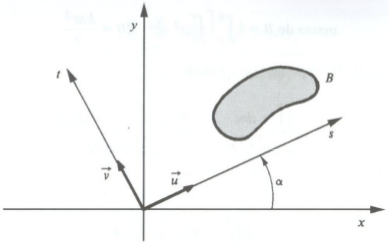
\includegraphics[width=7cm]{Selection_001.png} % leia abaixo
\end{figure}

$B_{xy}$ é o conjunto $B$ olhado em relação ao sistema $xy$ e $B_{st}$ é o conjunto $B$ olhado em relação ao sistema $st$. Observe que $B_{xy}$ é a imagem de $B_{st}$ pela mudança de coordenadas acima. Verifique que

	$$ 
		\begin{cases}
			x = s \ \cos \alpha - t \ \sin \alpha \\
			y = s \ \sin \alpha + t \ \cos \alpha
		\end{cases}
	$$
	
	e conclua que
	
	$$\dfrac{\partial (x,y) }{\partial (s,t)} = 1$$	
	
\item A integral Gaussiana é bastante conhecida pelas suas aplicações em fenômenos estatísticos e probabilísticos. Sua forma de resolução natural é bastante difícil, o que pede a utilização de ferramentas adicionais como cálculo numérico. No entanto, existe uma forma bastante simples de demonstrar que a integral abaixo é igual a 1. Considere a integral de densidade probabilidade abaixo:
	$$\integral_{-\infty}^{+\infty} \dfrac{1}{\sqrt{2 \pi \sigma^2}} e^{-(x - \mu)^2/2\sigma^2}  \, dx = 1$$
	
	Dica: Chame $(x - \mu)$ de $u$ e $\dfrac{1}{2\sigma^2}$ de $a$ e substitua dentro da integral:
	
	$$\dfrac{1}{\sqrt{2 \pi \sigma^2}} \integral_{-\infty}^{+\infty}  e^{-au^2}  \, du = 1$$
	
	Chame a integral $ \integral_{-\infty}^{+\infty}  e^{-au^2}  \, du $ de $I$ e resolva $I^2$. Considere $u$ como sendo uma variável qualquer.
	 	
	
	\end{enumerate}	
	
	
	
\end{document}